\section{Agent框架演进：从ReAct到智能操作系统}
\label{sec:agentevolution}

Agent框架（Agent Framework）是指围绕大语言模型构建的、使其能够自主规划、调用工具、管理状态并完成复杂任务的软件系统。
从2022年的研究原型到2025年的产品化运行时，Agent框架正在经历一次类似操作系统从单任务批处理到多任务分时、从无保护到有保护、从无治理到可信治理的系统性演进。
本节梳理这一演进的五个阶段，每个阶段从\textbf{核心架构特征}、\textbf{代表性系统及其具体做法}、以及\textbf{与经典操作系统演进的对应关系}三个维度展开分析。

图~\ref{fig_agent_timeline}展示了Agent框架五代演进的时间线。
\begin{figure}[htbp]
\centering
%% ── Gemini-generated image version (active) ──────────────────────────────────
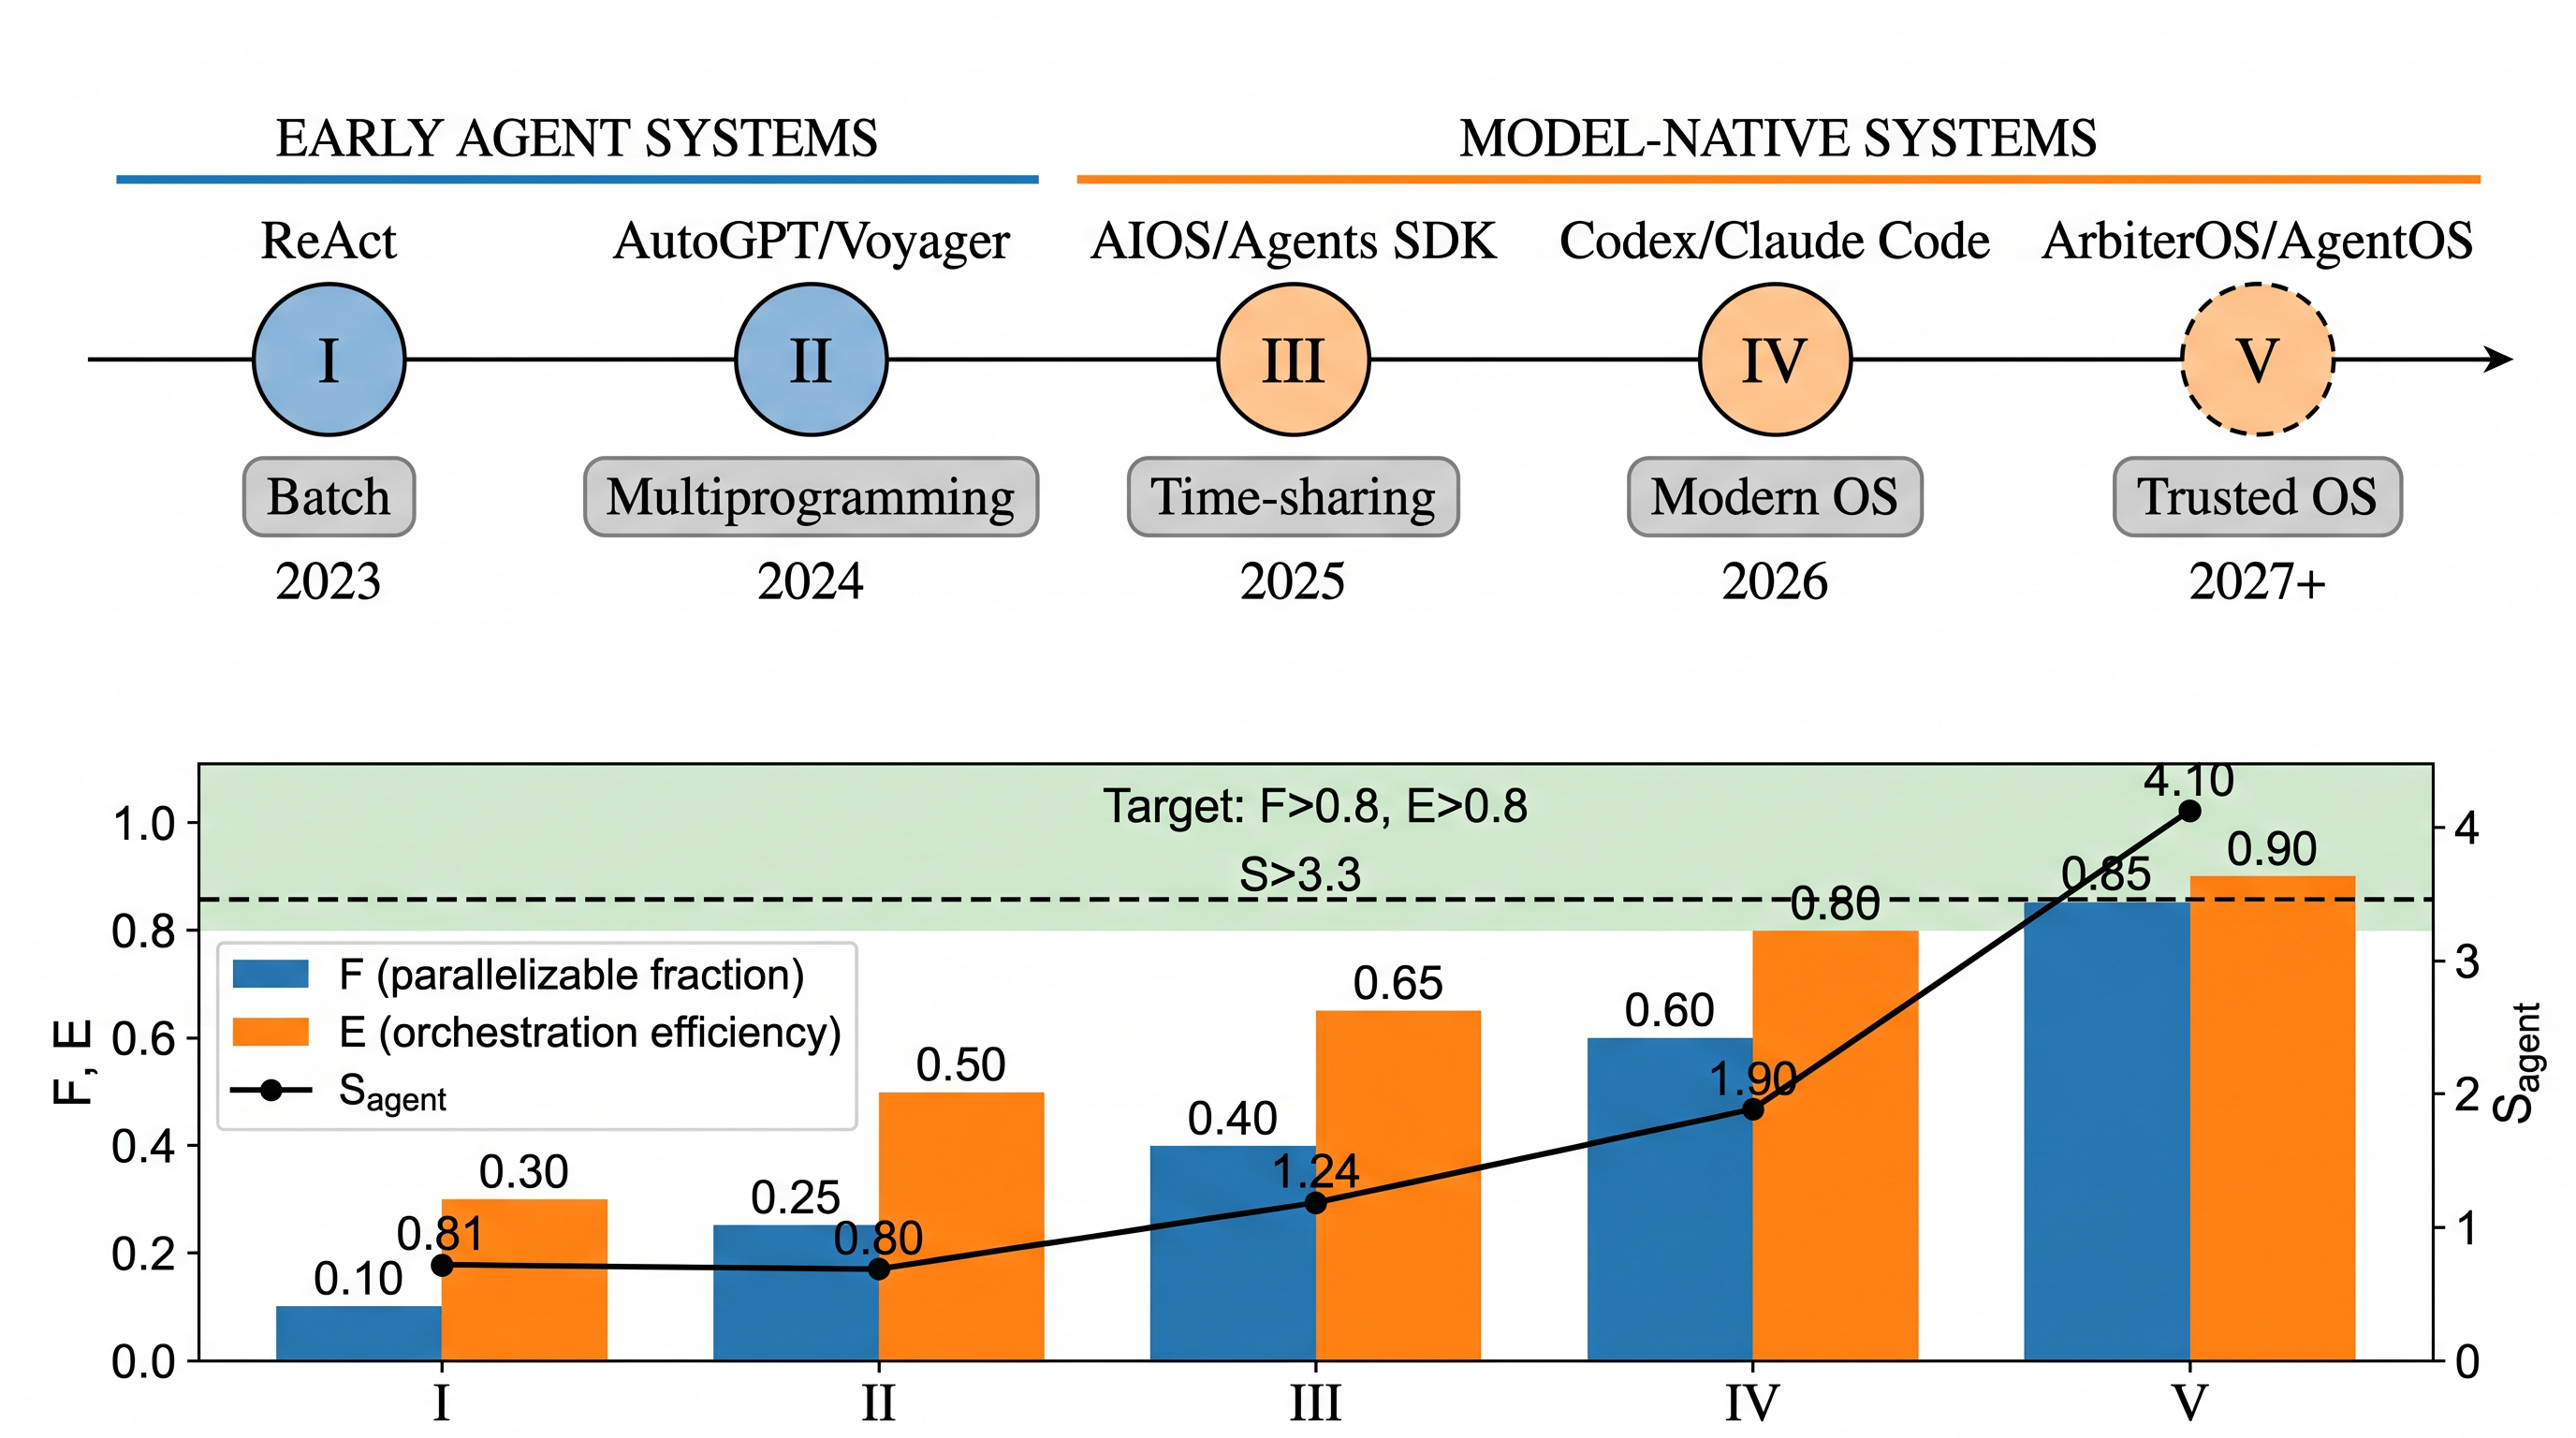
\includegraphics[width=0.95\textwidth]{figures/fig_agent_timeline_gemini.png}
%% ── Original TikZ version (commented out) ────────────────────────────────────
%\resizebox{0.95\textwidth}{!}{%
%\begin{tikzpicture}[
%    font=\sffamily,
%    >=Stealth,
%    milestone/.style={
%        circle,
%        minimum size=10mm,
%        inner sep=0pt,
%        line width=0.9pt,
%        font=\small\bfseries
%    },
%    early/.style={
%        milestone,
%        fill=softBlue,
%        draw=timelineBlue,
%        text=timelineBlue
%    },
%    native/.style={
%        milestone,
%        fill=softOrange,
%        draw=timelineOrange,
%        text=timelineOrange
%    },
%    future/.style={
%        native,
%        dashed
%    },
%    framework/.style={
%        align=center,
%        text width=29mm,
%        font=\small\bfseries,
%        text=timelineDark
%    },
%    oschip/.style={
%        rounded corners=2.5pt,
%        fill=softGray,
%        draw=timelineGray!65,
%        line width=0.45pt,
%        inner xsep=5pt,
%        inner ysep=2.6pt,
%        font=\scriptsize\itshape,
%        text=timelineDark,
%        align=center
%    },
%    year/.style={
%        font=\scriptsize\bfseries,
%        text=timelineGray!85!black
%    },
%    phase/.style={
%        font=\scriptsize\bfseries,
%        text=timelineDark
%    },
%    flow/.style={
%        -{Stealth[length=2.4mm,width=1.6mm]},
%        draw=timelineGray,
%        line width=0.95pt
%    }
%]

% Milestone nodes
%\node[early]  (g1) at (0.0,  0) {I};
%\node[early]  (g2) at (3.4,  0) {II};
%\node[native] (g3) at (6.8,  0) {III};
%\node[native] (g4) at (10.2, 0) {IV};
%\node[future] (g5) at (13.6, 0) {V};

% Evolution arrows
%\draw[flow] (g1.east) -- (g2.west);
%\draw[flow] (g2.east) -- (g3.west);
%\draw[flow] (g3.east) -- (g4.west);
%\draw[flow] (g4.east) -- (g5.west);

% Framework names
%\node[framework, above=5mm of g1] {ReAct};
%\node[framework, above=5mm of g2] {AutoGPT\\Voyager};
%\node[framework, above=5mm of g3] {AIOS\\Agents SDK};
%\node[framework, above=5mm of g4] {Codex\\Claude Code};
%\node[framework, above=5mm of g5] {ArbiterOS\\AgentOS};

% Operating-system analogies
%\node[oschip, below=8mm of g1] (o1) {Batch};
%\node[oschip, below=8mm of g2] (o2) {Multiprogramming};
%\node[oschip, below=8mm of g3] (o3) {Time-sharing};
%\node[oschip, below=8mm of g4] (o4) {Modern OS};
%\node[oschip, below=8mm of g5] (o5) {Trusted OS};

% Years
%\node[year, below=4mm of o1] {2023};
%\node[year, below=4mm of o2] {2024};
%\node[year, below=4mm of o3] {2025};
%\node[year, below=4mm of o4] {2026};
%\node[year, below=4mm of o5] {2027+};

% Phase headers
%\draw[timelineBlue, line width=0.95pt]
%    (-0.45, 2.28) -- (4.65, 2.28);
%\node[phase, text=timelineBlue]
%    at (2.10, 2.55) {EARLY AGENT SYSTEMS};

%\draw[timelineOrange, line width=0.95pt]
%    (5.95, 2.28) -- (14.05, 2.28);
%\node[phase, text=timelineOrange]
%    at (10.00, 2.55) {MODEL-NATIVE SYSTEMS};

%% ===========================================================
%% BOTTOM ROW: Quantitative F / E / S_agent chart (pgfplots)
%% ===========================================================
%% S_agent values computed via Law III:  S = 1/((1-F)+F/(N*E))
%%   Gen I:   N=1,  F=0.10, E=0.30 => S=0.81
%%   Gen II:  N=1,  F=0.25, E=0.50 => S=0.80
%%   Gen III: N=3,  F=0.40, E=0.65 => S=1.24
%%   Gen IV:  N=6,  F=0.60, E=0.80 => S=1.90
%%   Gen V:   N=10, F=0.85, E=0.90 => S=4.10

% ---- Left axis: F and E bars ----
%\begin{axis}[
%    name=barchart,
%    at={(-1.2,-8.0)},
%    anchor=north west,
%    width=15.6cm,
%    height=5.8cm,
%    ybar,
%    bar width=7pt,
%    ymin=0, ymax=1.08,
%    xmin=-0.5, xmax=4.5,
%    xtick={0,1,2,3,4},
%    xticklabels={I, II, III, IV, V},
%    xticklabel style={font=\sffamily\small\bfseries, color=timelineDark},
%    ytick={0,0.2,0.4,0.6,0.8,1.0},
%    yticklabels={0, 0.2, 0.4, 0.6, 0.8, 1.0},
%    yticklabel style={font=\sffamily\scriptsize, color=timelineDark},
%    ylabel={\small $F$,\; $E$},
%    ylabel style={font=\sffamily\small, color=timelineDark, at={(0.06,0.5)}},
%    axis y line*=left,
%    axis x line*=bottom,
%    enlarge x limits=0.15,
%    legend style={
%        at={(0.02,0.55)},
%        anchor=north west,
%        font=\sffamily\scriptsize,
%        draw=timelineGray!50,
%        fill=white,
%        fill opacity=0.9,
%        text opacity=1,
%        row sep=1pt,
%        /tikz/every even column/.append style={column sep=4pt}
%    },
%    tick style={draw=none},
%    major grid style={draw=timelineGray!20, line width=0.3pt},
%    ymajorgrids=true,
%    clip=false,
%]

% --- Target zone (F>0.8 and E>0.8 shaded region) ---
%\fill[green!12, opacity=0.5]
%    (axis cs:-0.5,0.8) rectangle (axis cs:4.5,1.08);
%\draw[green!50!black, densely dashed, line width=0.5pt]
%    (axis cs:-0.5,0.8) -- (axis cs:4.5,0.8);
% Label at top-right of green band, above the bars
%\node[font=\sffamily\tiny\itshape, text=green!40!black, anchor=north east]
%    at (axis cs:4.5,1.08) {Target: $F{>}0.8,\;E{>}0.8$};

% --- F bars (parallelizable fraction) ---
%\addplot[
%    fill=timelineBlue!55,
%    draw=timelineBlue,
%    line width=0.4pt
%] coordinates {
%    (0, 0.10)
%    (1, 0.25)
%    (2, 0.40)
%    (3, 0.60)
%    (4, 0.85)
%};
%\addlegendentry{$F$ (parallelizable fraction)}

% --- E bars (orchestration efficiency) ---
%\addplot[
%    fill=timelineOrange!55,
%    draw=timelineOrange,
%    line width=0.4pt
%] coordinates {
%    (0, 0.30)
%    (1, 0.50)
%    (2, 0.65)
%    (3, 0.80)
%    (4, 0.90)
%};
%\addlegendentry{$E$ (orchestration efficiency)}

%\end{axis}

% ---- Right axis: S_agent line ----
%\begin{axis}[
%    at={(barchart.south east)},
%    anchor=south east,
%    width=15.6cm,
%    height=5.8cm,
%    ymin=0, ymax=4.5,
%    xmin=-0.5, xmax=4.5,
%    xtick=\empty,
%    ytick={0,1,2,3,4},
%    yticklabels={$0$,$1$,$2$,$3$,$4$},
%    yticklabel style={font=\sffamily\scriptsize, color=timelineDark},
%    ylabel={\small $S_{\mathrm{agent}}$},
%    ylabel style={font=\sffamily\small, color=timelineDark, at={(0.96,0.5)}},
%    axis y line*=right,
%    axis x line=none,
%    enlarge x limits=0.15,
%    clip=false,
%    legend style={
%        at={(0.98,0.98)},
%        anchor=north east,
%        font=\sffamily\scriptsize,
%        draw=timelineGray!50,
%        fill=white,
%        fill opacity=0.9,
%        text opacity=1,
%        row sep=1pt
%    },
%]

% --- S_agent smooth line ---
%\addplot[
%    thick,
%    timelineDark,
%    mark=*,
%    mark size=2.5pt,
%    mark options={fill=timelineDark},
%    line width=1.1pt,
%    smooth
%] coordinates {
%    (0, 0.81)
%    (1, 0.80)
%    (2, 1.24)
%    (3, 1.90)
%    (4, 4.10)
%};
%\addlegendentry{$S_{\mathrm{agent}}$}

% --- S_agent value labels ---
%\node[font=\sffamily\tiny\bfseries, text=timelineDark, anchor=south]
%    at (axis cs:0,0.81) {0.81};
%\node[font=\sffamily\tiny\bfseries, text=timelineDark, anchor=south]
%    at (axis cs:1,0.80) {0.80};
%\node[font=\sffamily\tiny\bfseries, text=timelineDark, anchor=south]
%    at (axis cs:2,1.24) {1.24};
%\node[font=\sffamily\tiny\bfseries, text=timelineDark, anchor=south]
%    at (axis cs:3,1.90) {1.90};
%\node[font=\sffamily\tiny\bfseries, text=timelineDark, anchor=south]
%    at (axis cs:4,4.10) {4.10};

% --- Target S_agent dashed line at S=3.3 ---
%\draw[timelineDark, densely dotted, line width=0.6pt]
%    (axis cs:-0.5,3.3) -- (axis cs:4.5,3.3);
%\node[font=\sffamily\tiny\itshape, text=timelineDark, anchor=east]
%    at (axis cs:4.5,3.5) {$S{>}3.3$};

%\end{axis}

%\end{tikzpicture}}% end resizebox
\caption{Agent framework evolution from single-turn reasoning to model-native operating systems.
\textbf{Top:} representative frameworks with analogous OS milestones.
\textbf{Bottom:} quantitative trajectory of parallelizable fraction ($F$), orchestration efficiency ($E$), and agent speedup ($S_{\mathrm{agent}}$) per Law~III; green band marks the target regime ($F{>}0.8,\;E{>}0.8$).}
\label{fig_agent_timeline}
\end{figure}


%% ---------- 第一代 ----------
\subsection{第一代：执行范式确立（2022--2023）}

\paragraph{核心特征。}
第一代Agent框架确立了``推理--行动--观察''交织循环（Thought--Action--Observation loop）的基本范式。
在此之前，大语言模型的使用方式是``单轮问答''：用户给出提示，模型一次性返回回答，类似于向批处理系统提交一个作业并等待输出。
第一代框架打破了这一限制：模型不再是被动回答者，而是在循环中主动\textbf{推理}（分析当前状态并决定下一步）、\textbf{行动}（调用工具或执行操作）、\textbf{观察}（读取工具返回的结果），然后进入下一轮循环。

\paragraph{代表工作。}
ReAct\cite{yao2023react}是这一代的奠基工作。
它的核心做法是在提示模板中引入``Thought''字段，要求模型在每次调用工具前先显式输出推理过程。
例如，当用户问``莎士比亚最长的剧本是什么？''时，模型不是直接猜测答案，而是先输出``我需要搜索莎士比亚所有剧本的长度''，然后调用搜索工具，再根据搜索结果推理出最终答案。
这种``先想再做''的模式看似简单，却解决了大模型直接生成工具调用时常见的``幻觉式工具调用''问题。
Toolformer\cite{schick2023toolformer}则从另一个角度切入：让模型\textbf{自学}何时以及如何调用工具，通过在训练数据中注入工具调用示例来实现。

\paragraph{与OS演进的对应。}
这一代框架类似于1950年代的\textbf{单任务批处理系统}（如IBM 704的Fortran Monitor System）：系统一次只处理一个任务，做完再做下一个，没有并发、没有中断、没有状态保持。
ReAct的循环就是最简单的``取指--译码--执行''流水线，每次循环对应一个``指令周期''。
系统没有任何资源管理能力：没有任务调度（只有一个任务）、没有内存管理（上下文窗口就是全部``内存''）、没有I/O抽象（工具调用是硬编码的）。

%% ---------- 第二代 ----------
\subsection{第二代：持续多步代理（2023）}

\paragraph{核心特征。}
第二代框架的核心突破是\textbf{持续性}（persistence）和\textbf{自主目标分解}（autonomous goal decomposition）。
第一代框架中，每个用户提问触发一个独立的推理--行动循环；循环结束后，所有中间状态消失。
第二代框架允许Agent持续运行，自主将高层目标分解为子任务序列，维护跨步骤的中间状态，并在子任务之间传递信息。
这意味着Agent开始具备``工作记忆''的能力。

\paragraph{代表工作。}
AutoGPT\cite{autogpt_repo_2026}是第二代最知名的尝试。
用户给定一个高层目标（如``调研量子计算领域的最新进展并撰写报告''），AutoGPT自主将其分解为搜索论文、提取关键信息、组织大纲、撰写报告等子任务，并依次执行。
它引入了长期记忆（基于向量数据库）来存储跨步骤的中间结果，使Agent能``记住''之前做过什么。
然而，AutoGPT也暴露了第二代的核心问题：缺乏失败恢复机制，一旦某个子任务出错，整个链路容易陷入死循环或累积错误。
Voyager\cite{wang2023voyager}在Minecraft环境中做出了关键改进：引入了\textbf{技能库}（skill library）---将成功完成的子任务封装为可复用的``技能''，类似函数定义；以及\textbf{自动课程}（automatic curriculum）---根据当前能力自动生成下一步应学习的任务，类似教学大纲。
这使得Agent能够持续积累经验，而不是每次都从头开始。
BabyAGI则实现了更简洁的任务队列管理：维护一个待办任务列表，按优先级排序执行，并根据执行结果动态生成新任务。

\paragraph{与OS演进的对应。}
这一代框架类似于1960年代的\textbf{多道程序设计}（multiprogramming）：系统开始管理复杂的多步状态，任务之间可以共享和传递信息。
AutoGPT的任务队列就是最原始的``作业调度器''；Voyager的技能库类似于``可执行程序库''；BabyAGI的优先级排序类似于早期的``作业调度策略''。
但与成熟的OS相比，第二代框架缺少三个关键机制：\textbf{隔离}（不同任务之间可能相互干扰）、\textbf{调度}（没有抢占式调度，一个任务卡住会阻塞整个系统）、和\textbf{保护}（一个任务出错可能污染其他任务的状态）。

%% ---------- 第三代 ----------
\subsection{第三代：通用运行时（2023--2024）}

\paragraph{核心特征。}
第三代框架开始系统性地引入\textbf{调度}、\textbf{隔离}和\textbf{资源管理}能力，使Agent框架从``单脚本自动化工具''升级为``通用运行时平台''。
关键标志是：Agent不再只是一个串行执行的循环，而是可以被调度、被暂停、被恢复的``进程''；多个Agent可以并发运行且互不干扰；系统开始显式管理计算资源（推理次数、上下文空间、工具调用频率）。

\paragraph{代表工作。}
AIOS\cite{mei2024aios}构建了完整的Agent OS内核，其架构包含六个子系统：Agent Scheduler（负责多Agent的并发调度）、Context Manager（管理不同Agent的上下文隔离与共享）、Memory Manager（分层记忆管理）、 Tool Manager（工具注册与权限控制）、IO Manager（输入输出管理）和 Knowledge Manager（知识库管理）。
每个Agent被封装为一个``进程''，拥有独立的状态空间和资源预算。
OpenAI Agents SDK\cite{openai_codex_agentsdk_2026}则采取了更工程化的路线：将orchestration（编排）、state management（状态管理）、approvals（审批流）、handoffs（Agent间任务移交）与tracing（全链路追踪）做成代码优先（code-first）的运行时。
开发者可以用Python代码定义Agent的行为规范、权限边界和协作流程，而不是用提示模板来隐式地``编程''。
AutoGen\cite{wu2023autogen}提出了多Agent对话框架：多个Agent通过结构化的消息传递来协作完成复杂任务，每个Agent扮演不同角色（如程序员、测试员、项目经理），类似于多进程协作。

\paragraph{与OS演进的对应。}
这一代框架类似于1960--70年代的\textbf{分时操作系统}（Time-Sharing OS，如Multics和Unix）。
分时OS的核心突破是为每个用户（进程）提供独立的地址空间和公平的CPU时间片，使得多用户可以安全地共享同一台计算机。
AIOS的Agent Scheduler对应分时OS的进程调度器；Context Manager对应内存管理单元（MMU）的地址隔离；Tool Manager的权限控制对应Unix的文件权限系统。
Agents SDK的tracing机制则对应OS的\texttt{strace}/\texttt{auditd}系统调用追踪。

%% ---------- 第四代 ----------
\subsection{第四代：工程化操作系统（2024--2025）}

\paragraph{核心特征。}
第四代框架的核心标志是\textbf{面向真实软件工程环境的深度整合}。
前三代框架主要在实验室环境或受限场景中验证概念；第四代框架直面真实的代码库、真实的终端环境、真实的文件系统和真实的外部服务。
这意味着系统必须处理前几代可以回避的问题：大型代码仓库的上下文远超模型窗口、工具调用可能产生不可逆的副作用、并发编辑可能引发冲突、真实项目需要权限和审计。

\paragraph{代表工作。}
OpenAI Codex\cite{openai_codex_overview_2026}是一个运行在隔离沙箱中的云端代码Agent：它在独立的容器中checkout代码仓库，执行读写和运行命令，完成后提交差异（diff）供人类审查。
Codex引入了子Agent机制（subagents）：主Agent可以将子任务分派给专门的子Agent执行，子Agent在独立的沙箱中运行，结果经审批后合并---类似于Unix的\texttt{fork()}创建子进程。
Codex还支持技能包（skills）\cite{openai_codex_skills_2026}和项目级指令文件（AGENTS.md）\cite{openai_codex_agents_md_2026}，实现了跨项目的可复用配置。

Claude Code\cite{anthropic_claudecode_overview_2026}采取了互补的设计哲学：它运行在开发者本地终端，通过MCP协议\cite{mcp_intro_2026}连接外部工具，默认只读（除非用户显式授权写入），并支持自定义hooks来拦截和审计每一次工具调用\cite{anthropic_claudecode_security_2026}。
Claude Code的记忆系统\cite{anthropic_claudecode_memory_2026}区分了项目级记忆（\texttt{CLAUDE.md}，类似于系统配置文件）和用户级记忆（跨项目的个人偏好，类似于用户home目录下的点文件）。

OpenHands\cite{openhands_paper_2025}提供了开放的Agent平台，支持多种模型后端和沙箱环境，其OpenHands Index已成为评估代码Agent能力的标准基准之一。
OSWorld\cite{osworld2024}则从评估角度推动了这个方向：它构建了真实的操作系统环境（包含文件管理器、浏览器、终端等），要求Agent在真实的GUI环境中完成开放式任务，暴露了Agent在真实世界复杂性面前的局限性。
Devin\cite{devin2024cognition}进一步展现了第四代的工程化特征：作为一个``AI软件工程师''，它集成了代码编辑器、浏览器和终端，能够自主规划、编码、调试和部署。

\paragraph{与OS演进的对应。}
这一代框架类似于1980--90年代的\textbf{现代操作系统}（如Unix System V、Linux早期版本、Windows NT）。
现代OS的核心特征是处理真实世界的复杂性：多任务调度（CFS调度器\cite{linux_cfs_2026}）、虚拟内存与按需分页、网络协议栈、设备驱动框架、安全审计。
Codex的沙箱对应OS的进程隔离（每个子Agent在独立容器中运行，类似\texttt{chroot}或容器技术）；Claude Code的hooks对应Linux的LSM（Linux Security Modules）安全钩子；Codex的审批机制对应Unix的\texttt{sudo}权限提升；OpenHands的多模型后端对应OS的硬件抽象层（HAL）。

%% ---------- 第五代 ----------
\subsection{第五代：治理化操作系统（2025--至今）}

\paragraph{核心特征。}
第五代框架的核心突破是\textbf{将安全和治理从事后补丁升级为体系结构的第一性设计原则}。
前四代框架的安全措施是``加法式''的：先让Agent能工作，再加沙箱、加审批、加日志。
第五代框架反过来：先定义安全边界和治理规则，再在边界内赋予Agent行动能力。
这种范式的转变类似于操作系统从``可用''到``可信''的转折---正如Multics在1960年代就引入了环保护（ring protection）和强制访问控制（mandatory access control），但直到SELinux和Capability-based Security普及后，安全才真正成为OS体系结构的有机组成部分\cite{ostep_2023}。

\paragraph{代表工作。}
ArbiterOS\cite{arbiteros2025}明确提出了``Probabilistic CPU + Deterministic Governor/Kernel''的分层架构：底层的LLM是概率式处理器，负责``能做什么''；上层的governor是确定性控制器，负责``应该做什么''。
governor通过策略文件（policy specification）定义Agent的行为边界，类似于OS内核通过系统调用表和权限位定义进程的能力范围。

AgentOS\cite{agentos2025}引入了受结构化操作系统逻辑（structured operating system logic）约束的推理内核（reasoning kernel），从token级别的上下文管理出发，逐步构建出系统级的智能行为。
其核心思想是：Agent的推理过程不应该是不可控的``黑箱循环''，而应该像OS内核一样，通过结构化的抽象和接口来管理。

UFO$^2$\cite{ufo2_2025}面向桌面环境，将Desktop AgentOS组织为三层结构：HostAgent（顶层协调者，类似于init进程）、AppAgent（每个应用程序一个，类似于服务进程）、和GUI--API action layer（底层操作接口，类似于驱动层）。
这种分层使得Agent对不同应用程序的操作可以被独立管理和审计。

Aura\cite{aura2025}则在移动端实现了安全优先的Agent OS架构：System Agent（系统级Agent，拥有最高权限）、Sandboxed App Agents（每个应用一个，运行在沙箱中，类似于Android的应用沙箱）、和Agent Kernel（Agent内核，负责权限仲裁和资源分配）。
Aura特别强调了移动端环境的独特风险：语义输入污染（通过恶意输入劫持Agent行为）、记忆taint传播（被污染的记忆影响后续所有操作）、以及跨应用权限泄露。

CaMeL\cite{debenedetti2025camel}从安全原则出发，提出了基于能力（capability）的安全模型来防御提示注入攻击。
其核心思想借鉴自操作系统中的capability-based security：Agent不能直接执行任何有副作用的操作，而必须通过一个确定性的capability manager来获取``临时通行证''。
每个通行证只授权一个特定操作（如``只读文件X''），而不是授予全局权限。
这类似于Unix从``root/非root''的粗粒度权限模型，向POSIX capability和SELinux的细粒度权限模型的演进。

IronClaw\cite{ironclaw2025}系统性地论证了为什么AI Agent需要像操作系统一样被保护。
它指出，传统软件安全假设``代码是确定性的、行为是可预测的''，但Agent的行为由概率式模型驱动，攻击面从``代码漏洞''扩展到了``语义漏洞''---攻击者可以通过自然语言提示来劫持Agent的行为，而不需要利用任何代码缺陷。

OWASP在2025年底发布的\textbf{Agentic Applications Top 10}\cite{owasp_agentic2026}进一步系统化了这些威胁：Agent Goal Hijack（目标劫持）、Tool Misuse \& Exploitation（工具滥用）、Identity \& Privilege Abuse（身份与权限滥用）等十大风险类别，为第五代框架的安全设计提供了分类学基础。

\paragraph{与OS演进的对应。}
这一代框架对应操作系统从``可用''到``可信''的转折期。
在经典OS历史上，Unix V6（1975年）是一个``可用但不安全''的系统：没有内存保护，任何进程都可以读写任何内存地址；没有权限分离，root用户拥有不受限制的权力。
随着网络和多用户环境的发展，安全性从``可选功能''变为``必要基础''，导致了Multics的环保护、SELinux的强制访问控制、以及现代微内核（如seL4）的形式化验证\cite{ostep_2023}。
第五代Agent框架正在经历同样的转折：安全性不再只是``加个沙箱''，而是需要从体系结构层面重新设计Agent的权限模型、审计机制和失败恢复策略。

%% ---------- 演进的量化视角 ----------
图~\ref{fig_gen_matrix}总结了五代框架在六个体系结构维度上的能力成熟度。
\begin{figure}[htbp]
    \centering
    \resizebox{\textwidth}{!}{%
    \begin{tikzpicture}[
        cell/.style={
            minimum width=2.4cm, minimum height=1.0cm,
            align=center, font=\scriptsize,
            inner sep=2pt,
        },
        rowlabel/.style={
            % 【修复点】：将过宽的宽度大幅缩小至 2.8cm，彻底解决边框太宽和重叠问题
            minimum width=2.8cm, minimum height=1.0cm,
            text width=2.5cm, align=left, font=\small\bfseries,
            inner sep=4pt,
        },
        collabel/.style={
            minimum width=2.4cm, minimum height=0.9cm,
            align=center, font=\small\bfseries,
            inner sep=2pt,
        },
    ]
    
    % ── Capability columns ────────────────────────────────────────────────────────
    \def\cols{{"Task\\Decomp.", "Concurrency\\(F)", "Orchestration\\Eff.~(E)", "State\\Persist.", "Isolation\\/ Sandbox", "Security\\/ Govern."}}
    \def\ncols{6}
    
    % ── Color helper: 0=none, 1=low, 2=mid, 3=high ──────────────────────────────
    % 0 → white, 1 → 25%, 2 → 55%, 3 → 85% of modelnative
    \def\fillcol#1{%
        \ifnum#1=0 white\fi%
        \ifnum#1=1 modelnative!20\fi%
        \ifnum#1=2 modelnative!50\fi%
        \ifnum#1=3 modelnative!85\fi%
    }
    \def\txtcol#1{%
        \ifnum#1=0 gray!40\fi%
        \ifnum#1=1 modelnative!60!black\fi%
        \ifnum#1=2 modelnative!70!black\fi%
        \ifnum#1=3 white\fi%
    }
    \def\levelstr#1{%
        \ifnum#1=0 ---\fi%
        \ifnum#1=1 Low\fi%
        \ifnum#1=2 Medium\fi%
        \ifnum#1=3 High\fi%
    }
    
    % Data: rows = Gen I..V, each row = 6 values (0-3)
    % Gen I  (ReAct)
    \def\rowA{0,0,3,0,0,0}
    % Gen II (AutoGPT)
    \def\rowB{1,0,2,1,0,0}
    % Gen III (AIOS/SDK)
    \def\rowC{2,2,2,2,1,1}
    % Gen IV (Codex/Claude Code)
    \def\rowD{3,3,2,3,3,2}
    % Gen V (ArbiterOS/AURA)
    \def\rowE{3,3,3,3,3,3}
    
    \def\rowlabels{{"Gen~I\\(ReAct)", "Gen~II\\(AutoGPT)", "Gen~III\\(AIOS)", "Gen~IV\\(Codex)", "Gen~V\\(ArbiterOS)"}}
    \def\sublabels{{"2022--23", "2023", "2023--24", "2024--25", "2025--"}}
    
    % ── Draw column headers ───────────────────────────────────────────────────────
    \foreach \j/\lbl in {
        0/Task\\Decomp.,
        1/Concurrency\\$(F)$,
        2/Orchestration\\Eff.~$(E)$,
        3/State\\Persist.,
        4/Isolation\\/ Sandbox,
        5/Security\\/ Govern.}
    {
        \node[collabel, draw=gray!30, fill=gray!10]
            at ({3.9 + \j*2.4}, 0.5) {\lbl};
    }
    
    % Row label header
    % 【修复点】：X坐标整体向左平移至 1.3，与右侧列（起点 2.7）完美断开
    \node[rowlabel, draw=gray!30, fill=gray!10, minimum height=0.9cm]
        at (1.3, 0.5) {Generation};
    
    % ── Helper macro to draw one cell ────────────────────────────────────────────
    \newcommand{\drawcell}[3]{% #1=col(0-5), #2=row(0-4), #3=value(0-3)
        \pgfmathsetmacro\vint{int(#3)}%
        \ifnum\vint=0 \def\fc{white}\def\tc{gray!35}\fi%
        \ifnum\vint=1 \def\fc{modelnative!20}\def\tc{modelnative!65!black}\fi%
        \ifnum\vint=2 \def\fc{modelnative!50}\def\tc{modelnative!80!black}\fi%
        \ifnum\vint=3 \def\fc{modelnative!85}\def\tc{white}\fi%
        \node[cell, draw=gray!25, fill=\fc, text=\tc, minimum height=1.0cm]
            at ({3.9 + #1*2.4}, {-#2*1.0 - 0.5})
            {\ifnum\vint=0 ---\fi%
             \ifnum\vint=1 Low\fi%
             \ifnum\vint=2 Medium\fi%
             \ifnum\vint=3 High\fi};%
    }
    
    % ── Draw row labels ───────────────────────────────────────────────────────────
    \foreach \i/\rlab/\rsub in {
        0/{Gen~I}/{\footnotesize 2022--23},
        1/{Gen~II}/{\footnotesize 2023},
        2/{Gen~III}/{\footnotesize 2023--24},
        3/{Gen~IV}/{\footnotesize 2024--25},
        4/{Gen~V}/{\footnotesize 2025--Present}%
    }{
        \node[rowlabel, draw=gray!20, fill=gray!5, minimum height=1.0cm]
            at (1.3, {-\i*1.0 - 0.5})
            {\textbf{\rlab}\\[1pt]\rsub};
    }
    
    % ── Draw cells: \drawcell{col}{row}{value} ────────────────────────────────────
    % Gen I  (ReAct)
    \drawcell{0}{0}{0} \drawcell{1}{0}{0} \drawcell{2}{0}{3}
    \drawcell{3}{0}{0} \drawcell{4}{0}{0} \drawcell{5}{0}{0}
    
    % Gen II (AutoGPT/Voyager)
    \drawcell{0}{1}{1} \drawcell{1}{1}{0} \drawcell{2}{1}{2}
    \drawcell{3}{1}{1} \drawcell{4}{1}{0} \drawcell{5}{1}{0}
    
    % Gen III (AIOS/SDK)
    \drawcell{0}{2}{2} \drawcell{1}{2}{2} \drawcell{2}{2}{2}
    \drawcell{3}{2}{2} \drawcell{4}{2}{1} \drawcell{5}{2}{1}
    
    % Gen IV (Codex/Claude Code)
    \drawcell{0}{3}{3} \drawcell{1}{3}{3} \drawcell{2}{3}{2}
    \drawcell{3}{3}{3} \drawcell{4}{3}{3} \drawcell{5}{3}{2}
    
    % Gen V (ArbiterOS/AgentOS)
    \drawcell{0}{4}{3} \drawcell{1}{4}{3} \drawcell{2}{4}{3}
    \drawcell{3}{4}{3} \drawcell{4}{4}{3} \drawcell{5}{4}{3}
    
    % ── Legend (centred under table) ─────────────────────────────────────────────
    % 【修复点】：整体微调图例的坐标，使其严格居中对齐整个表格
    \node[font=\scriptsize, text=gray!60, anchor=east] at (5.7, -5.65) {Maturity:};
    \foreach \v/\lbl in {0/None, 1/Low, 2/Medium, 3/High} {
        \ifnum\v=0\def\fc{white}\def\tc{gray!40}\fi
        \ifnum\v=1\def\fc{modelnative!20}\def\tc{modelnative!65!black}\fi
        \ifnum\v=2\def\fc{modelnative!50}\def\tc{modelnative!80!black}\fi
        \ifnum\v=3\def\fc{modelnative!85}\def\tc{white}\fi
        \node[draw=gray!30, fill=\fc, text=\tc,
              minimum width=1.5cm, minimum height=0.55cm,
              font=\scriptsize, rounded corners=2pt]
            at ({6.7 + \v*1.9}, -5.65) {\lbl};
    }
    
    \end{tikzpicture}
    }% end resizebox
    \caption{Capability maturity matrix across the five generations of agent framework evolution. Each cell reflects the maturity level of a key architectural dimension: \textit{None} (---) through \textit{High}. The progressive darkening from Generation~I to Generation~V illustrates the systematic increase in both the parallelisable fraction~$F$ and the orchestration efficiency~$E$ captured by Law~III.}
    \label{fig_gen_matrix}
    \end{figure}

\subsection{从启发式III看五代演进}

从第~\ref{sec:laws}节提出的Agent加速比启发式（启发式III）的视角看，五代演进对应着$F$（可分解比例）和$E$（编排效率）的逐步提升。

回顾启发式III的形式：
\begin{equation}
\label{eq:agent_law_review}
S_{\mathrm{agent}} = \frac{1}{(1-F) + \dfrac{F}{N \cdot E}}
\end{equation}
其中$F \in [0,1]$是任务中可以被并行分解的比例，$N$是可调度的Agent数量，$E \in (0,1]$是编排效率（1表示无开销，0表示开销吞噬全部并行收益）。

\textbf{具体数值分析}
图~\ref{fig:gen_trajectory}绘制了五代框架的$F$、$E$和$S_{\mathrm{agent}}$估计值。

% ---------------------------------------------------------------------------
% Five-Generation Quantitative Trajectory: F, E, S across Gen I–V
% fig:gen_trajectory
% ---------------------------------------------------------------------------
\begin{figure}[htbp]
\centering
\resizebox{0.88\textwidth}{!}{%
\begin{tikzpicture}
\small
\begin{groupplot}[
    group style={
        group size=3 by 1,
        horizontal sep=2.2cm,
    },
    width=5.0cm,
    height=5.2cm,
    grid=major,
    grid style={gray!18},
    tick label style={font=\footnotesize},
    label style={font=\small},
    xtick={1,2,3,4,5},
    xticklabels={I,II,III,IV,V},
    xlabel style={font=\small},
    ylabel style={font=\small},
    xmin=0.5, xmax=5.5,
    axis lines=left,
    every axis plot/.append style={thick, mark=*, mark size=2.2pt},
    enlargelimits=0.12,
    legend style={
        font=\scriptsize,
        at={(0.5,-0.32)},
        anchor=north,
        legend columns=1,
        draw=gray!40,
        rounded corners=2pt,
    },
]

%% (a) Parallelizable Fraction F
\nextgroupplot[
    title style={font=\small\bfseries, at={(0.5,1.06)}},
    title={(a) Parallelizable Fraction $F$},
    xlabel={Generation},
    ylabel={$F$},
    ymin=0, ymax=1.05,
    ytick={0,0.2,0.4,0.6,0.8,1.0},
]
\addplot[blue!70!black, mark=*]
    coordinates {(1,0.00)(2,0.15)(3,0.30)(4,0.50)(5,0.72)};
% target line
\addplot[red!60!black, dashed, no marks, domain=0.5:5.5] {0.8};
\addlegendentry{$F$ (estimated)}
\addlegendentry{Target $F>0.8$}
% annotations (shifted left)
\node[font=\tiny, blue!60!black, anchor=east] at (axis cs:0.9, 0.05) {${\approx}0$};
\node[font=\tiny, blue!60!black, anchor=east] at (axis cs:1.85, 0.20) {$0.15$};
\node[font=\tiny, blue!60!black, anchor=east] at (axis cs:2.85, 0.35) {$0.30$};
\node[font=\tiny, blue!60!black, anchor=east] at (axis cs:3.85, 0.53) {$0.50$};
\node[font=\tiny, blue!60!black, anchor=east] at (axis cs:4.85, 0.73) {$0.72$};

%% (b) Orchestration Efficiency E
\nextgroupplot[
    title style={font=\small\bfseries, at={(0.5,1.06)}},
    title={(b) Orchestration Efficiency $E$},
    xlabel={Generation},
    ylabel={$E$},
    ymin=0, ymax=1.05,
    ytick={0,0.2,0.4,0.6,0.8,1.0},
]
\addplot[orange!80!black, mark=square*]
    coordinates {(1,1.00)(2,0.90)(3,0.70)(4,0.50)(5,0.65)};
\addplot[red!60!black, dashed, no marks, domain=0.5:5.5] {0.8};
\addlegendentry{$E$ (estimated)}
\addlegendentry{Target $E>0.8$}
\node[font=\tiny, orange!70!black] at (axis cs:1, 0.88) {$1.0$};
\node[font=\tiny, orange!70!black] at (axis cs:2, 1) {$0.9$};
\node[font=\tiny, orange!70!black] at (axis cs:3, 0.58) {$0.7$};
\node[font=\tiny, orange!70!black] at (axis cs:4, 0.38) {$0.5$};
\node[font=\tiny, orange!70!black] at (axis cs:5, 0.5) {$0.65$};

%% (c) Agent Speedup S
\nextgroupplot[
    title style={font=\small\bfseries, at={(0.5,1.06)}},
    title={(c) Agent Speedup $S_{\mathrm{agent}}$},
    xlabel={Generation},
    ylabel={$S_{\mathrm{agent}}$},
    ymin=0, ymax=4.0,
    ytick={0,1,2,3,4},
]
\addplot[red!70!black, mark=triangle*, mark size=2.5pt]
    coordinates {(1,1.00)(2,1.00)(3,1.27)(4,1.60)(5,2.10)};
\addplot[red!50!black, dashed, no marks, domain=0.5:5.5] {3.3};
\addlegendentry{$S_{\mathrm{agent}}$}
\addlegendentry{Target $S>3.3$}
\node[font=\tiny, red!65!black] at (axis cs:1, 1.3) {$1.0$};
\node[font=\tiny, red!65!black] at (axis cs:2, 1.3) {$1.0$};
\node[font=\tiny, red!65!black] at (axis cs:3, 1.7) {$1.27$};
\node[font=\tiny, red!65!black] at (axis cs:4, 2.0) {$1.60$};
\node[font=\tiny, red!65!black] at (axis cs:5, 2.5) {$2.10$};

\end{groupplot}
\end{tikzpicture}}%
\caption{Quantitative trajectory of agent framework parameters across five generations, estimated from Law~III ($S_{\mathrm{agent}} = 1/((1-F)+F/(N{\cdot}E))$ with representative $N$ values per generation). (a)~Parallelizable fraction $F$ grows from near zero (Gen~I serial loop) to ${\approx}0.72$ (Gen~V governed OS). (b)~Orchestration efficiency $E$ initially near~1 (trivial single-agent overhead) but dips in Gen~IV due to sandbox isolation and approval overhead, then recovers in Gen~V with governance-first design. (c)~Resulting speedup $S_{\mathrm{agent}}$ rises from $1.0\times$ to ${\approx}2.1\times$, still well below the target $3.3\times$ that requires $F>0.8$ and $E>0.8$ simultaneously. Dashed red lines mark the target thresholds.}
\label{fig:gen_trajectory}
\end{figure}


第一代（ReAct）：$F \approx 0$（任务不分解，单Agent串行执行），$N=1$，$E \approx 1$（无编排开销），$S_{\mathrm{agent}} \approx 1$。这对应``单处理器无并行''的状态。
第二代（AutoGPT/Voyager）：$F \approx 0.1$--$0.2$（少量子任务可以被分离），$N=1$（仍然是单Agent），$E \approx 0.9$，$S_{\mathrm{agent}} \approx 1$。分解能力初现，但编排开销不大，因为只有一个Agent。
第三代（AIOS/Agents SDK）：$F \approx 0.3$（中等分解能力），$N \approx 2$--$4$（开始支持多Agent），$E \approx 0.7$（调度和上下文切换引入显著开销），$S_{\mathrm{agent}} \approx 1/(0.7 + 0.3/2.8) \approx 1.27$。多Agent开始带来加速，但编排开销抵消了部分收益。
第四代（Codex/Claude Code）：$F \approx 0.5$（面向真实软件工程的代码任务有较高的可分解性），$N \approx 4$--$8$（子Agent并发），$E \approx 0.5$（沙箱隔离、审批流程、状态同步带来显著开销），$S_{\mathrm{agent}} \approx 1/(0.5 + 0.5/4) \approx 1.6$。加速比显著提升，但编排开销仍是瓶颈。

第五代（ArbiterOS/CaMeL/IronClaw）：$F \approx 0.72$（治理优先设计使更广泛的任务分解成为可能），$N \approx 6$（成熟的多Agent并发），$E \approx 0.65$（通过结构化策略执行和能力令牌部分回收治理开销），$S_{\mathrm{agent}} \approx 1/(0.28 + 0.72/3.9) \approx 2.1$。
$E$相对于第四代的部分回升反映了从临时沙箱向基于能力的原则性安全的转变，这减少了冗余的权限检查。然而，$F$和$E$仍低于实现$3.3\times$加速目标所需的$0.8$阈值。

第四代系统的执行时间跨度也正在从分钟级向小时级扩展：Rakuten的工程师测试Claude Code在vLLM项目（1250万行代码）上自主运行7小时完成激活向量提取，达到99.9\%数值精度\cite{anthropic2026agenticreport}。
这种长期自主执行引入了新的体系结构挑战——跨小时的KV缓存持久化、检查点/恢复协议和资源管理——正是Agent运行时类比操作系统的有力支撑。

真正的``模型原生操作系统''需要$F > 0.8$且$E > 0.8$，此时$S_{\mathrm{agent}} > 1/(0.2 + 0.8/8) \approx 3.3$，这意味着既要有好的任务分解（高$F$），又要有低的编排开销（高$E$）。

GAIA\cite{gaia2023}、$\tau$-bench\cite{taubench2024}和SWE-bench\cite{swebench2023}的最新结果提醒我们，当前系统离这个目标还有相当距离。
以SWE-bench Verified为例，截至2025年末，最佳Agent系统在该基准上的通过率约为70--75\%---这意味着在四分之一的真实软件工程任务中，Agent仍然无法正确分解和执行。
在$\tau$-bench中，Agent在与真实用户进行多轮交互时的表现更加不稳定，因为用户指令的歧义性和环境的动态性进一步降低了$F$和$E$。

%% ============================================================
